\subsection{Proceso Interno 14: Formar Siguiente Población}

\subsubsection{Objetivo del Proceso}
El propósito principal es construir la población para la próxima iteración del algoritmo genético, combinando:
\begin{itemize}
    \item Los $k$ mejores individuos (élite) de \texttt{Poblacion\_Actual}
    \item Los $(N - k)$ mejores descendientes
\end{itemize}
Manteniendo el tamaño poblacional $N$.

\subsubsection{Entradas Principales}
\begin{itemize}
    \item \textbf{Población Actual}:
    \begin{itemize}
        \item $N$ individuos ${\{x_i, F_p^i\}}_{i=1}^N$
    \end{itemize}
    \item \textbf{Descendencia}:
    \begin{itemize}
        \item $N$ individuos nuevos ${\{x'_j, F_p^j\}}_{j=1}^N$
    \end{itemize}
    \item \textbf{Parámetros}:
    \begin{itemize}
        \item $k \in \mathbb{N}$ (tamaño de élite)
        \item $N \in \mathbb{N}$ (tamaño población)
    \end{itemize}
\end{itemize}

\subsubsection{Sub-pasos Secuenciales}
Este apartado es proporcionado para profundizar y describir de forma textual cada paso contenido dentro del diagrama del proceso descrito en la figura~\ref{fig:process_diagram14}
\subsubsection*{1. Ordenar Poblaciones}
\begin{itemize}
    \item $\texttt{Poblacion\_Actual} \leftarrow \text{sort\_asc}(\{F_p^i\})$
    \item $\texttt{Descendencia} \leftarrow \text{sort\_asc}(\{F_p^j\})$
\end{itemize}

\subsubsection*{2. Inicializar Población Siguiente}
\begin{itemize}
    \item Crear \texttt{Poblacion\_Siguiente} $= \emptyset$
\end{itemize}

\subsubsection*{3. Aplicar Elitismo}
\begin{equation*}
    \texttt{Poblacion\_Siguiente} \leftarrow \begin{cases}
    \text{primeros } k \text{ de } \texttt{Poblacion\_Actual} & \text{si } k > 0 \\
    \emptyset & \text{si } k = 0
    \end{cases}
\end{equation*}

\subsubsection*{4. Completar con Descendencia}
\begin{align*}
    \text{num\_a\_copiar} &= N - |\texttt{Poblacion\_Siguiente}| \\
    \texttt{Poblacion\_Siguiente} &\leftarrow \texttt{Poblacion\_Siguiente} \cup \{\text{primeros num\_a\_copiar de Descendencia}\}
\end{align*}

\subsubsection*{5. Verificación Final}
\begin{itemize}
    \item Asegurar $|\texttt{Poblacion\_Siguiente}| = N$
    \item Manejo de errores (relleno adicional si es necesario)
\end{itemize}

\subsubsection{Lógica Interna y Decisiones}
\begin{itemize}
    \item \textbf{Elitismo condicional}:
    \begin{itemize}
        \item $k > 0 \Rightarrow$ preservar élite
        \item $k = 0 \Rightarrow$ reemplazo completo
    \end{itemize}

    \item \textbf{Selección por fitness}:
    \begin{itemize}
        \item Ordenamiento basado en $F_p$ ascendente
        \item $\text{num\_a\_copiar} = N - k$ garantiza tamaño poblacional
    \end{itemize}
\end{itemize}

\subsubsection{Manejo de Datos Específico}
\begin{itemize}
    \item \textbf{Entradas}:
    \begin{itemize}
        \item Dos poblaciones ordenables por $F_p$
        \item Parámetros $k$, $N$ de configuración
    \end{itemize}

    \item \textbf{Intermedios}:
    \begin{itemize}
        \item Poblaciones ordenadas
        \item Contador num\_a\_copiar
    \end{itemize}

    \item \textbf{Salida}:
    \begin{itemize}
        \item \texttt{Poblacion\_Siguiente} con $N$ individuos
    \end{itemize}
\end{itemize}

\subsubsection{Salidas Principales}
\begin{itemize}
    \item \textbf{Población siguiente}:
    \begin{itemize}
        \item $\{\text{élite}\} \cup \{\text{mejores descendientes}\}$
        \item Lista para próxima iteración del algoritmo
    \end{itemize}
\end{itemize}

\subsubsection{Interacciones Internas}
\begin{itemize}
    \item \textbf{Con módulo de ordenación}: Clasificación por $F_p$
    \item \textbf{Con gestor de poblaciones}: Fusión controlada de individuos
    \item \textbf{Con ConfigurationData}: Lectura de $k$ y $N$
\end{itemize}

\subsubsection{Diagrama del Proceso}
\begin{figure}[H]
    \centering
    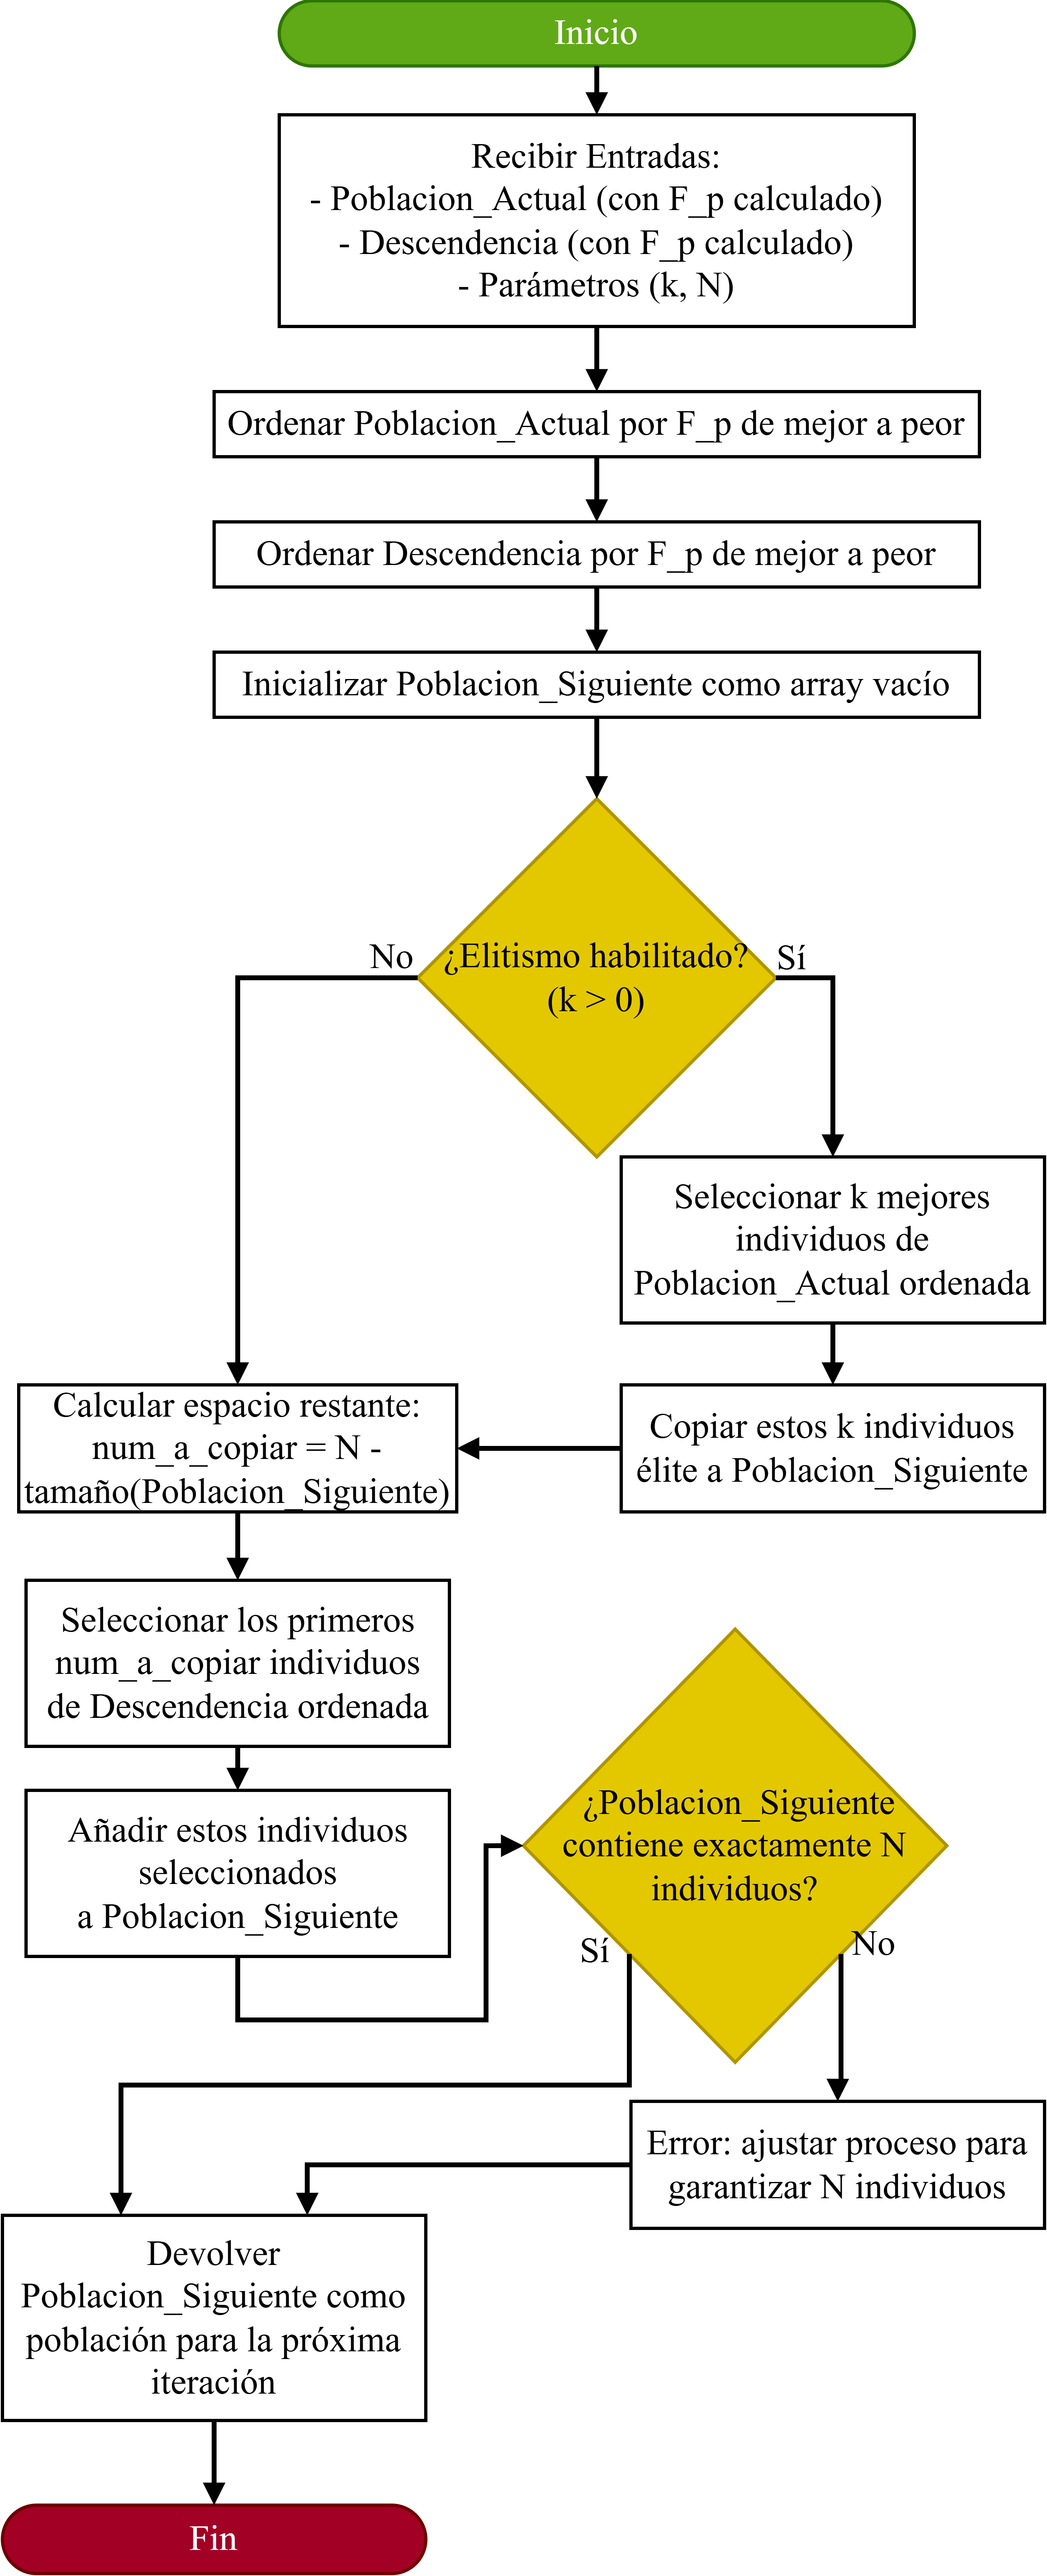
\includegraphics[width=\textwidth]{img/Analisis/DiagramaProcesos/DiagramaProceso14_SeleccionIndividuos.png}
    \caption{Diagrama de Proceso Interno 14: Selección de Individuos}%
    \label{fig:process_diagram14}
\end{figure}
